\documentclass[a4paper,11pt]{article}

\usepackage[english]{babel}
%\usepackage[portuguese]{babel}
\usepackage[T1]{fontenc}
\usepackage{amsmath, amssymb}
\usepackage{graphicx}

\usepackage{color}
\usepackage{listings}

\lstset{
    backgroundcolor=\color[rgb]{0.86,0.88,0.93},
    language=R, keywordstyle=\color[rgb]{0,0,1},
    basicstyle=\footnotesize \ttfamily,breaklines=true,
    escapeinside={\%*}{*)}
}

\begin{document}

%%%%%%%%%% Title %%%%%%%%%%%
\begin{figure}[!h] 
\includegraphics [scale=0.3] {Course-name} \end{figure}
%\pagestyle{empty}
{\Large \noindent \bf Homework II} 

\vskip0.8cm

%%%%%%%%%% Content starts here %%%%%%%%%%%
{\Large \noindent \bf Exercise 1} \hfill					20 Points\\

\noindent The unit steps responses of two systems $A$ and $B$ are recorded and reported in the files {\tt HW2\_ex1\_dataA.txt} and  {\tt HW2\_ex1\_dataB.txt}, respectively. In each file, the first column gives the time vector $t$ and the second column gives the output response $y$. \\

\noindent It is required to:
\begin{enumerate}
\item Load the data in Matlab/Octave and plot the two responses.
\item Estimate the transfer functions for the system $A$ and $B$. 
\item Compare your estimated systems with the ones provided in the data.
\end{enumerate}

\vskip0.5cm

{\Large \noindent \bf Exercise 2} \hfill					25 Points\\

\noindent Find the transfer function, $T(s)=C(s)/R(s)$, for the system in Figure (\ref{fig:ex2}), using the following methods:

\begin{enumerate}
\item Block diagram reduction.
\item Matlab/Octave. Use the following transfer functions:
\begin{align*}
G1(s)& =\cfrac{1}{(s+7)}, \quad G2(s)=\cfrac{1}{(s^2 + 2 s+3)},\\
G3(s)& =\cfrac{1}{(s+4}, \quad G4(s) =\cfrac{1}{s},\\
G5(s)& =\cfrac{5}{(s+ 7)}, \quad G6(s) =\cfrac{1}{(s^2 + 5s + 10)},\\
G7(s)&= \cfrac{3}{(s+ 2)}, \quad G8(s) = \cfrac{1}{(s + 6)}. 
\end{align*}
{\bf Hint}: Use the {\tt append} and {\tt connect} commands in Matlab/Octave Control System Toolbox/Package.
\end{enumerate}

\begin{figure}[ht!] \begin{center}
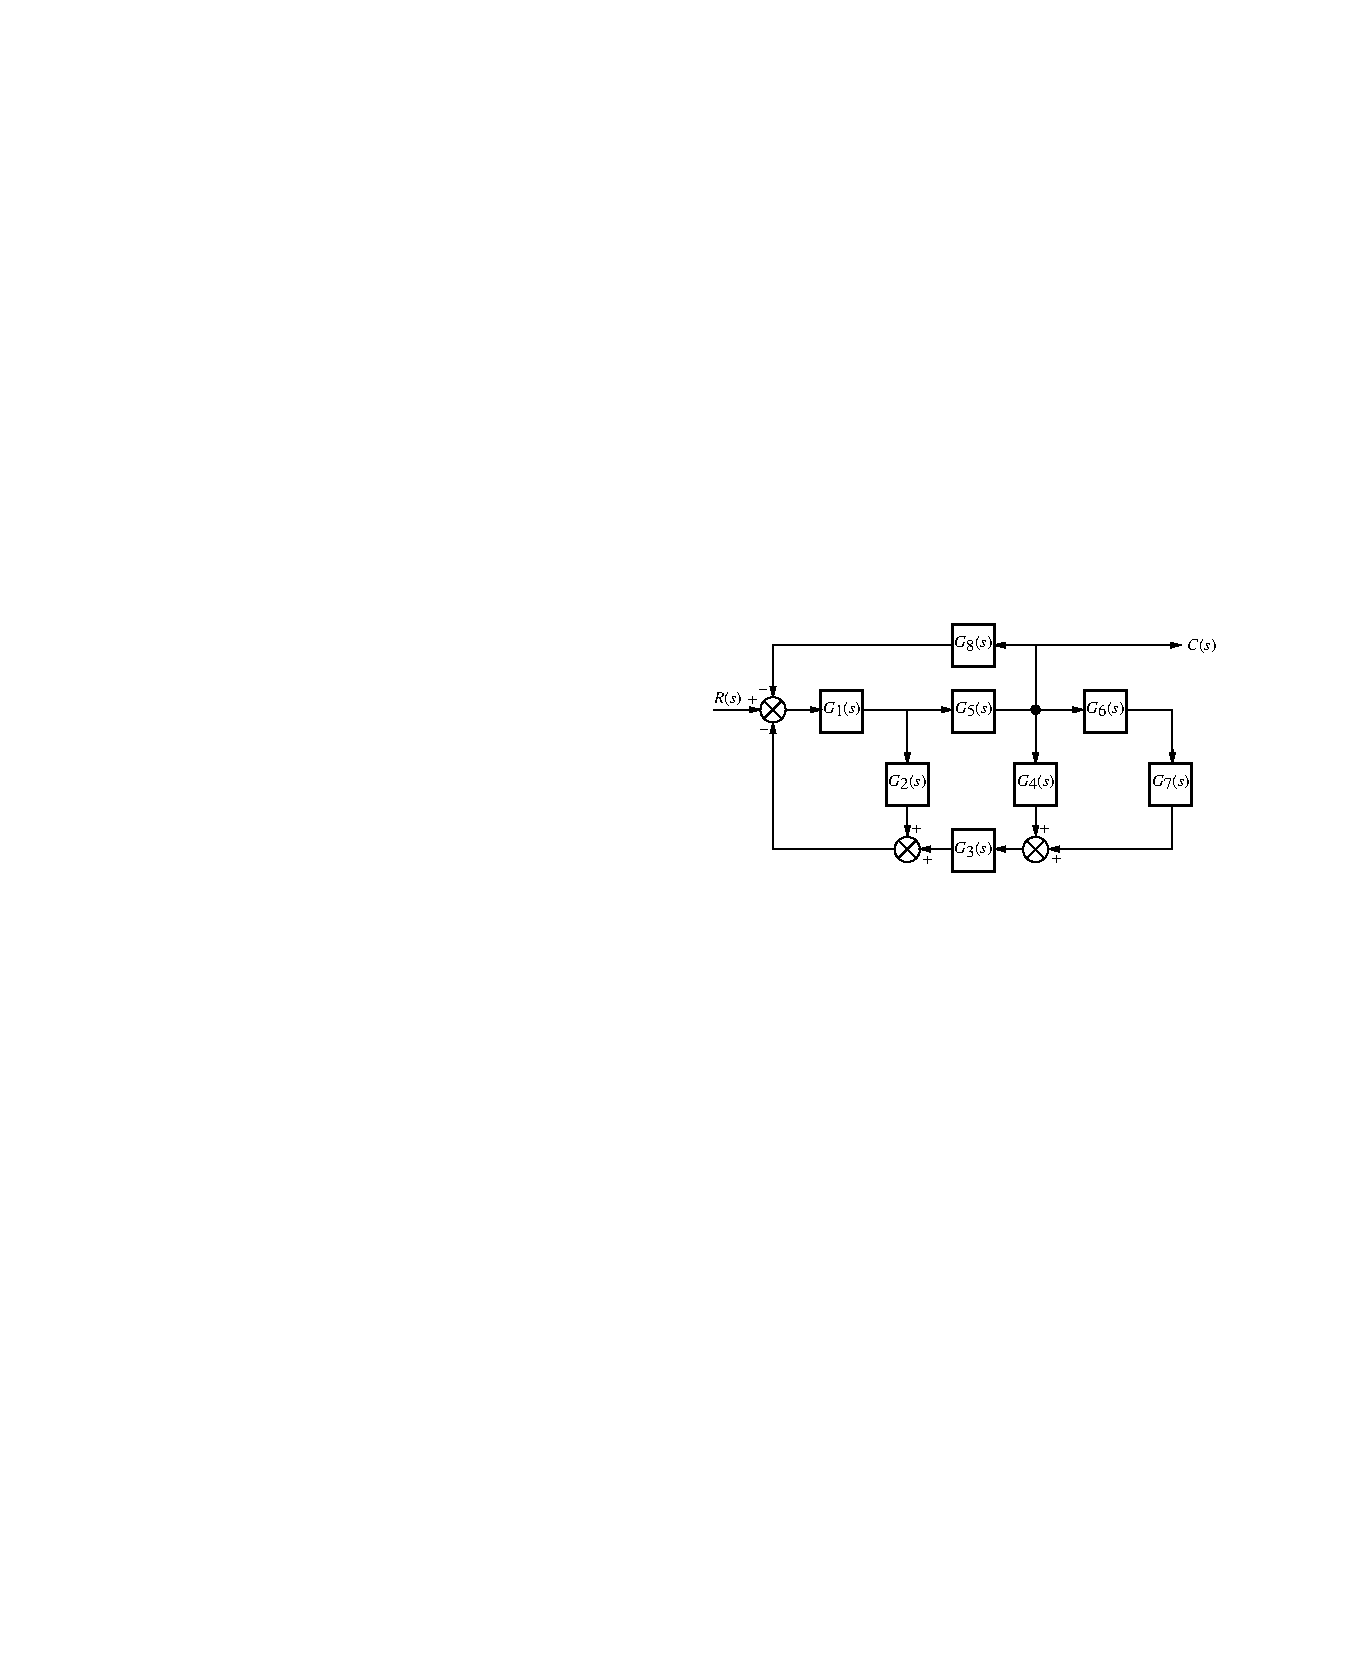
\includegraphics[width=1\textwidth]{Figures/blocks_ex}
 \caption{Block diagram for Exercise 2.} \label{fig:ex2}
\end{center} \end{figure}

\vskip0.5cm

{\Large \noindent \bf Exercise 3} \hfill					20 Points\\

\noindent The system in state space given in (\ref{eq:ss}) represents the forward path of a unity feedback system. 
\begin{align}
\begin{split}
\mathbf{\dot{x}} & =\begin{bmatrix}
0 & 1 & 0\\
0 & 0 & 1\\
-3 & -4 & -5\\
\end{bmatrix}
\mathbf{x}+\begin{bmatrix}
0 & 0 & 1
\end{bmatrix}
u \\
y & = \begin{bmatrix}
0 & 1 & 1
\end{bmatrix}
\mathbf{x}
\end{split}
\label{eq:ss}
\end{align}

\noindent Constructing the Routh table in Matlab/Octave, use the Routh-Hurwitz criterion to determine if the closed loop is stable.

\vskip0.5cm
{\Large \noindent \bf Exercise 4} \hfill					35 Points\\

\noindent  For a system with the state and output equations given in (\ref{eq:ex3}):
\begin{align}
\begin{split}
\dot{x}(t)& =x^2(t)-u(t)x(t)-2u(t)\\
y(t)& =x^3(t)+u^3(t)
\end{split}
\label{eq:ex3}
\end{align}  

\begin{enumerate}
\item Calculate the state and output equilibrium points when $u(t)=u_{eq}=1$.
\item Define the linearised system around the equilibrium points and analise the stability of the system.
\item \label{ex3:item3} Compare the linearised and nonlinear system responses $\delta y(t)$ for an input $\delta u(t)=A cos(2t)$, whit $A=0.1$ applied at $t=0$.
\item \label{ex3:item4} {\bf Extra (5 points)}: Investigate how the responses differ when the input amplitude assumes the values $[0.05, 0.15, 0.2]$. 
\item {\bf Extra (5 points)}: Calculate the error between linearised and nonlinear system in point (\ref{ex3:item3}) and point (\ref{ex3:item4}). Comment your findings.
\end{enumerate}

\noindent{\bf Hint}: Use the command {\tt ode45} to simulate the nonlinear system.

\end{document}